\documentclass[10pt,titlepage]{article}
\usepackage[english]{babel}
\usepackage[utf8]{inputenc}
\usepackage{algorithm}
\usepackage[noend]{algpseudocode}
\usepackage{amsmath,amsfonts,amsthm}
\usepackage{spverbatim}
\usepackage{listings}
\usepackage{xcolor}
\usepackage{pgfplots}
\usepackage[letterpaper, margin=1.25in]{geometry}
\usepackage{titlesec}
\usepackage{fancyhdr}
\usepackage{hyperref}
\usepackage{graphicx}
\usetikzlibrary{trees}
\usepackage[normalem]{ulem}
\useunder{\uline}{\ul}{}

\lstdefinestyle{mystyle}{
	keywordstyle=\color{blue},
	commentstyle=\color{red},
	stringstyle=\color{violet},
	basicstyle=\fontsize{12}{12},
	columns=fullflexible,
	breaklines=true
}

\titleformat{\section}
{\normalfont\Large\bfseries}{\thesection}{1em}{}[{\titlerule[0.8pt]}]
\lstset{style=mystyle}

\title{Implementation Design}
\author{Seth Williams, Abraham Sharum, Parker Fletcher, Bryson Dye \\\\ \\ Due Date: October 9, 2025 \\ Class: CS 40003 - Software Engineering}

\begin{document}
	\pagestyle{fancy}
	\fancyhead{}
	\fancyhead[LE,LO]{\textbf{CS 40003 - Software Engineering}}
	\fancyhead[RO,RE]{\textbf{Implementation Design}}
	\fancyfoot{}
	\fancyfoot[CE,CO]{\textbf{\thepage}}
	
	\maketitle
	
	\section*{GitTea Repository Structure}
	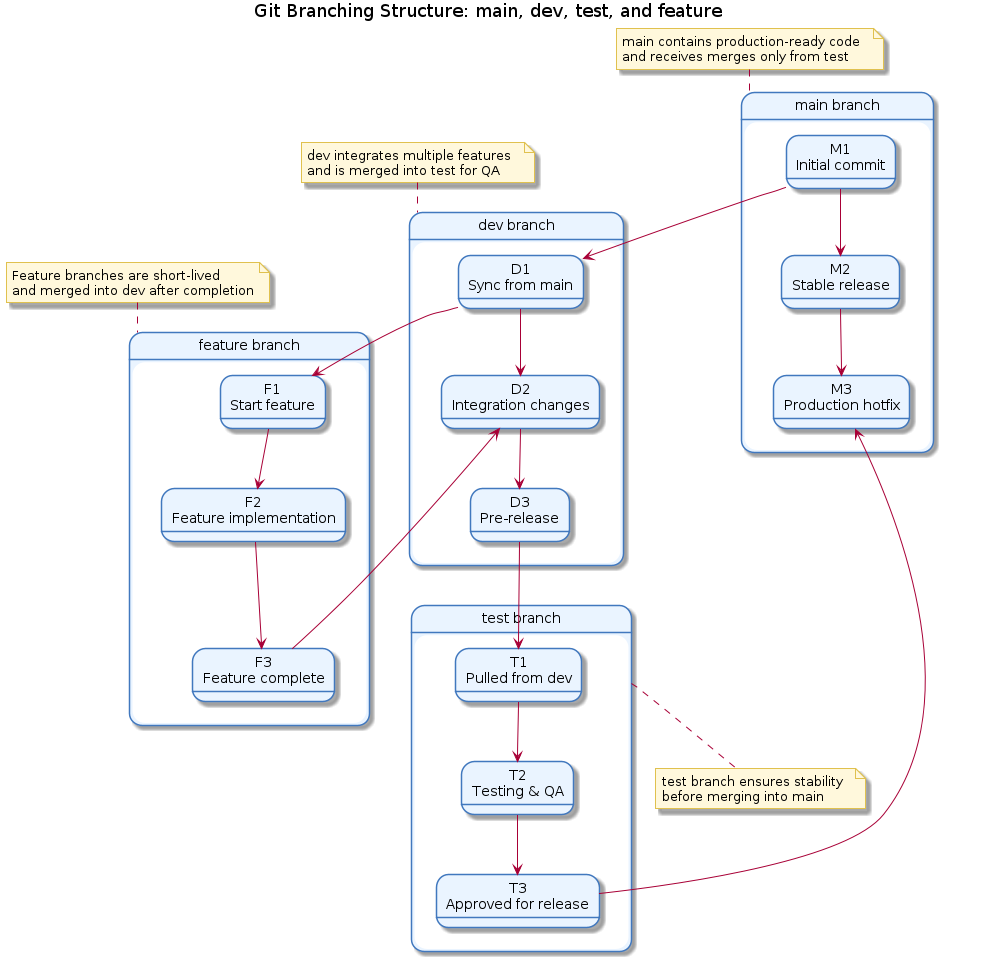
\includegraphics[width=1\textwidth]{branches.png}
	
	\clearpage
	
	\section*{Coding Standards}
	
	\subsection*{PHP Standards}
	\begin{itemize}
		\item Opening braces are on the same line as declarations
		\item One class per file, file name matches class name
		\item Naming conventions:
		\begin{itemize}
			\item Classes: \texttt{PascalCase} 
			\item Methods: \texttt{camelCase} 
			\item Variables: \texttt{\$camelCase}
			\item Constants: \texttt{UPPER\_SNAKE\_CASE}
		\end{itemize}
	\end{itemize}
	
	\subsection*{HTML Standards}
	\begin{itemize}
		\item Use lowercase for all element and attribute names
		\item Indent nested elements by 2 spaces
		\item Use double quotes for all attribute values
		\item Use semantic tags for structure: \texttt{<header>}, \texttt{<main>}, \texttt{<footer>}, \texttt{<section>}.
		\item Always include alt text for images
		\item Close all elements, including void elements like \texttt{<br>} and \texttt{<img>}
		\item Separate structure (HTML), style (CSS), and logic (JavaScript)
	\end{itemize}
	
	\subsection*{JavaScript Standards}
	\begin{itemize}
		\item Indentation: 2 spaces
		\item Use \texttt{const} and \texttt{let} instead of \texttt{var}
		\item Use single quotes for strings
		\item Always use semicolons
		\item Use strict equality (\texttt{===} and \texttt{!==})
		\item Avoid global variables
		\item Naming conventions:
		\begin{itemize}
			\item Variables and functions: \texttt{camelCase}
			\item Classes and constructors: \texttt{PascalCase}
			\item Constants: \texttt{UPPER\_SNAKE\_CASE}
		\end{itemize}
		\item Use meaningful variable names, avoid single letter identifiers outside of indices 
	\end{itemize}
	
	\subsection*{SQL Standards}
	\begin{itemize}
		\item Use uppercase for all SQL keywords 
		\item Use lowercase with underscores for table and column names
		\item Use consistent indentation and line breaks for readability:
		\begin{itemize}
			\item Each major clause (\texttt{SELECT}, \texttt{FROM}, \texttt{WHERE}, \texttt{GROUP BY}, etc.) on a new line
			\item Align columns in \texttt{SELECT} statements vertically
		\end{itemize}
		\item Always end statements with a semicolon
		\item Avoid using \texttt{SELECT *}, explicitly list required columns
		\item Use aliases with the \texttt{AS} keyword for clarity
		\item Use foreign key constraints for relational integrity
	\end{itemize}
	
	\subsection*{Security Standards}
	\begin{itemize}
		\item Validate all user input on both client and server sides
		\item Use prepared statements to prevent SQL injection
		\item Hash all stored passwords
		\item Use HTTPS for secure communication between clients and servers
		\item Store API keys and credentials in environment variables, not in the repository
		\item Limit user permissions and apply role-based access control
		\item Implement secure session handling with timeouts and token regeneration
		\item Do not expose detailed error messages to users
	\end{itemize}
	
\end{document}
